% Drawing 74/01-4 -- folder 74, batch 01, archive page 20 (PDF page 21).
% Transcription: À droite de $E^{\varepsilon}$, une rangée de points encadrée dont les deux derniers sont reliés à un point inférieur en forme de V, et sous elle une rangée de points pointillée terminée par un segment vertical.
% Kind: rows of points (framed row, V). Method 2 (schematic redraw from the facsimile). Status: ok.
% Notes: Right of E^epsilon: a framed row of points, the last two joined in bold to a lower point (the V); under it a dotted row ending in a vertical stroke.
% Coordinates: 1 unit = 1 mm = 1/100 of the crop width (bbox in page fractions: [0.6, 0.07, 0.9, 0.17]).
% Redrawn by Claude (claude-opus-5-5), issue #73, 2026-11-07; not checked by a human; not compiled (no TeX in the session).
% Rights: reproduces part of the work -- behind RENDER_TRANSCRIPTS, never published by itself.
\documentclass[tikz,border=3pt]{standalone}
\usepackage{amsmath,amssymb}
\usetikzlibrary{patterns,arrows.meta}
\tikzset{pencil/.style={black!45}, struck/.style={black!35}, mark/.style={circle,draw,inner sep=1.3pt}, pt/.style={circle,fill,inner sep=0.9pt}, opt/.style={circle,draw,fill=white,inner sep=1.1pt}}
\begin{document}
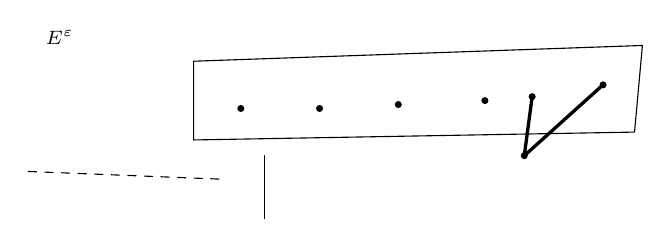
\begin{tikzpicture}[x=1mm,y=1mm,line cap=round,line join=round,font=\scriptsize]
\node[inner sep=1pt] at (14,-20) {\scriptsize $E^{\varepsilon}$};
\draw (31,-23) -- (88,-21) -- (87,-32) -- (31,-33) -- cycle;
\node[pt] at (37,-29) {};
\node[pt] at (47,-29) {};
\node[pt] at (57,-28.5) {};
\node[pt] at (68,-28) {};
\draw[very thick] (74,-27.5) -- (73,-35) -- (83,-26);
\node[pt] at (74,-27.5) {};
\node[pt] at (73,-35) {};
\node[pt] at (83,-26) {};
\draw[dashed] (10,-37) -- (35,-38);
\draw (40,-35) -- (40,-43);
\end{tikzpicture}
\end{document}
